\documentclass[10pt]{article}
\usepackage[utf8]{inputenc}
\usepackage{url}
\usepackage{hyperref}
\usepackage{amsmath}
\usepackage{amsfonts}
\usepackage{amssymb}
\usepackage{graphicx}
\graphicspath{ {./images/} }
\usepackage{float}
\usepackage{lipsum}
\usepackage{sectsty}
\usepackage{tikz}
\sectionfont{\centering}
\usepackage{multicol}
\usepackage{xcolor}
\usepackage{natbib}
\usepackage{graphicx}
\usepackage{listings}
\usepackage{xcolor}
\usepackage{pgfplots}
\usepackage[font=small]{caption}
\addtolength{\abovecaptionskip}{-3mm}
\addtolength{\textfloatsep}{-5mm}
\setlength\columnsep{20pt}

\usepackage[a4paper,left=1.50cm, right=1.50cm, top=2cm, bottom=3cm]{geometry}


\author{}

\title{\Large{Design and Analysis of Algorithms Assignment - 6}}
\begin{document}
	\begin{center}
		{\Large \textbf{Design and Analysis of Algorithms Assignment - 6}}\\
		\vspace{1em}
		{\large Department of Information Technology}\\
		\vspace{1em}
		\large{Indian Institute of Information Technology - Allahabad, India}\\
		\vspace{1em}
		\large{Sainath Reddy \hspace{10em} Jyoti Verma \hspace{10em} Krishna Kaipa}
		\large{IIT2019201 \hspace{10.5em} IIT2019202 \hspace{10.5em} IIT2019203}
		
		\vspace{2.5em}
	\end{center}
	
\begin{multicols*}{2}

    \textbf{\emph{{Abstract}: Transportation problem is a linear problem of cost minimization in the transportation from a set of suppliers to a set of destinations. This paper discusses north-west corner solution for the given problem as well as propose an alternative approach. The time complexity of this approach is measured to be O(N).}}\\
	
	\textbf{\emph{{Index Terms}: Arrays, Minimum cost, \\}}


\section*{INTRODUCTION}
 
Transportation problem is a linear problem in which goods are transported from a set of sources to a set of destinations subject to the supply and demand of the sources and destination respectively such that the total cost of transportation is minimized. There are several methods to solve this problem and we will be discussing the north-west corner approach.

This report further contains:
\begin{itemize}
\item 	Algorithm  Designs
\item 	Algorithm  Analysis
\item 	Experimental Study and Profiling
\item 	Conclusion
\item 	References
\item 	Appendix
\end{itemize}

\section*{ALGORITHM DESIGN}
The North-West Corner Rule is a method adopted to compute the initial feasible solution of the transportation problem. The name North-west corner is given to this method because the basic variables are selected from the extreme left corner. The prerequisite condition for solving the transportation problem is that demand should be equal to the supply. In case the demand is more than supply, then dummy origin is added to the table.

\paragraph{Algorithmic Steps:}

We basically select the north-western most corner available, compute the supply and demand operations and move to the next box accordingly.

\begin{enumerate}
\item We take input for the size of the cost matrix.
\item We store n X n randomly generated values in an 2D array.
\item We then elect the north-west or extreme left corner of the matrix, assign as many units as possible to the cell, within the supply and demand constraints. 
\item Either the demand is satisfied or the supply is finished or both. Based on either of these 3 possibilities, we either move 1 column across (if the demand is satisfied) or 1 row downwards(if the supply is finished) or both 1 row down and 1 column across (if supply and demand are equal).
\item This process is repeated until the the demand and supply are saturated and compute the total cost associated with the transport.
\end{enumerate}

Presenting below is the pseudo code for the above given algorithm.

\lstset { %
    language=C++,
    backgroundcolor=\color{black!5},
    basicstyle=\footnotesize,
}

\begin{lstlisting}
    
Int:
Function main()
    int n
    print Enter n:
    Input n
    
    arr :array
    supply :array
    demand :array
    
    print Generated post matrix:
    loop i=0 to n with i++
        arr[i][j] = rand() % 9 + 1
        print arr[i][j]
        
    loop i=0 to n with i++
        demand[i] = rand() % 250 + 1
        supply[i] = demand[i]
    
    shuffle(demand)
    
    print Demands:
    loop i=0 to n with i++
        print demand[i]
        
    print Supply:
    loop i=0 to n with i++
        print supply[i]
    
    i :int
    j :int
    cost :int
    
    while(i != n && j!= n)
        if(demand[i]==supply[j])
        
		 cost+= demand[i]*arr[i][j]
		 i++
		 j++
		 demand[i] = 0
		 supply[j] = 0
		 	
		else if(demand[i]<supply[j])
		
		 supply[j]-=demand[i]
		 cost+= demand[i]*arr[i][j]
		 demand[i] = 0
		 i++
				
		else if(demand[i]>supply[j])
		
		 demand[i]-=supply[j];
		 cost+= supply[i]*arr[i][j];
		 supply[j]=0;
		 j++;
    
    cost += demand[n-1] * arr[i-1][j-1]
    demand[n-1] -= supply[n-1]
    supply[n-1] = 0
	
	print cost
    return 0


\end{lstlisting}
    

\section*{ALGORITHM ANALYSIS} 
	
\paragraph{APRIORI ANALYSIS :}
This is the analysis performed prior to running in a stage where the function is defined using a theoretical model. Therefore, complexity is determined by just examining the algorithm rather than running it on a particular system with a different memory,processor, and compiler. So,as we discussed under the heading complexity analysis we arrived at the conclusion that the best time complexity is O(n) and the space complexity O(n).

Time complexity Derivation: Since we run a single loop to compute the cost, the time complexity is O(n).

\paragraph{Time Analysis:}Following is the graph representing the time complexity of the algorithm.\\\\\\
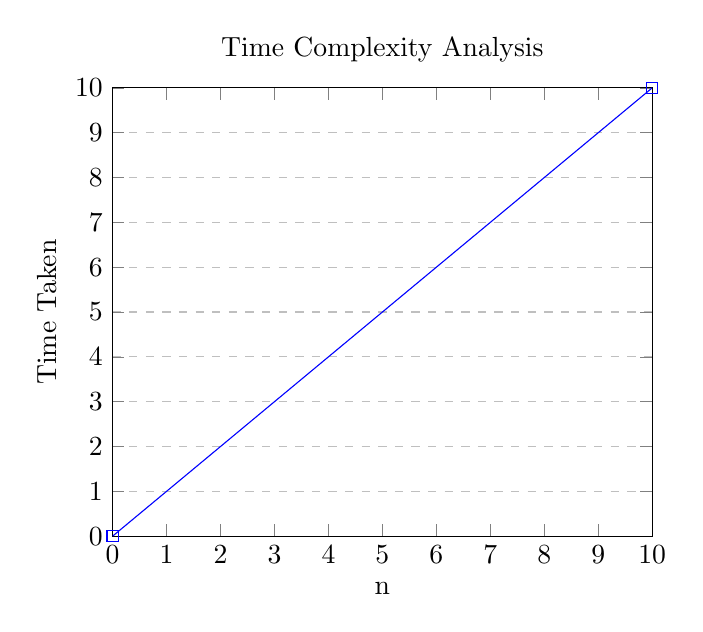
\begin{tikzpicture}
\begin{axis}[
    title={Time Complexity Analysis},
    xlabel={n},
    ylabel={Time Taken},
    xmin=0, xmax=10,
    ymin=0, ymax=10,
    xtick={0,1,2,3,4,5,6,7,8,9,10},
    ytick={0,1,2,3,4,5,6,7,8,9,10},
    legend pos=north west,
    ymajorgrids=true,
    grid style=dashed,
]

\addplot[
    color=blue,
    mark=square,
    ]
    coordinates {
    (0,0)(10,10)
    };
    
\end{axis}
\end{tikzpicture}

By the experimental analysis, we found that in  case of optimized approach, on increasing the number of numbers the graph is strictly increasing. Thus the overall time increases with an increase in size.

\paragraph{Space Analysis:}Following is the graph representing the space complexity of the algorithm.\\\\
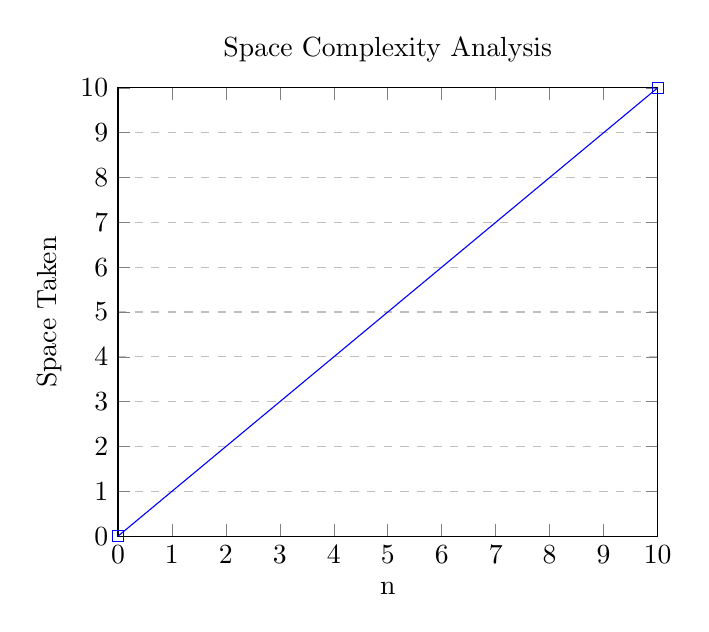
\begin{tikzpicture}
\begin{axis}[
    title={Space Complexity Analysis},
    xlabel={n},
    ylabel={Space Taken},
    xmin=0, xmax=10,
    ymin=0, ymax=10,
    xtick={0,1,2,3,4,5,6,7,8,9,10},
    ytick={0,1,2,3,4,5,6,7,8,9,10},
    legend pos=north west,
    ymajorgrids=true,
    grid style=dashed,
]

\addplot[
    color=blue,
    mark=square,
    ]
    coordinates {
    (0,0)(10,10)
    };
    
\end{axis}
\end{tikzpicture}

By the experimental analysis, we found that in case of optimized approach, on increasing the number of numbers the graph is strictly increasing. Thus the overall space increases with an increase in size.\\

\paragraph{APOSTERIORI ANALISIS:}
Aposteriori analysis of an algorithm means we per- form analysis of an algorithm only after running it on a system. It directly depends on the system and changes from system to system. So for the a aposteriori analysis of the algorithm,we have run our code on the compiler and get values of the time.

\section*{Experimental Analysis}
In the following table some cases are plotted for the algorithm on our local machine,
\begin{center}
 \begin{tabular}{||c | c||} 
 \hline
 n & Time Taken (in ms) \\ [0.5ex] 
 \hline\hline
 10 & 0.004 \\ 
 \hline
 100 & 0.0049 \\
 \hline
 1000 & 0.025 \\
 \hline
 5000 & 0.068 \\
 \hline
 10000 & 0.12 \\
 \hline
 50000 & 0.71 \\
 \hline
 100000 & 1.32 \\
 \hline
 1000000 & 11.2 \\ [1ex] 
 \hline
\end{tabular}
\end{center}

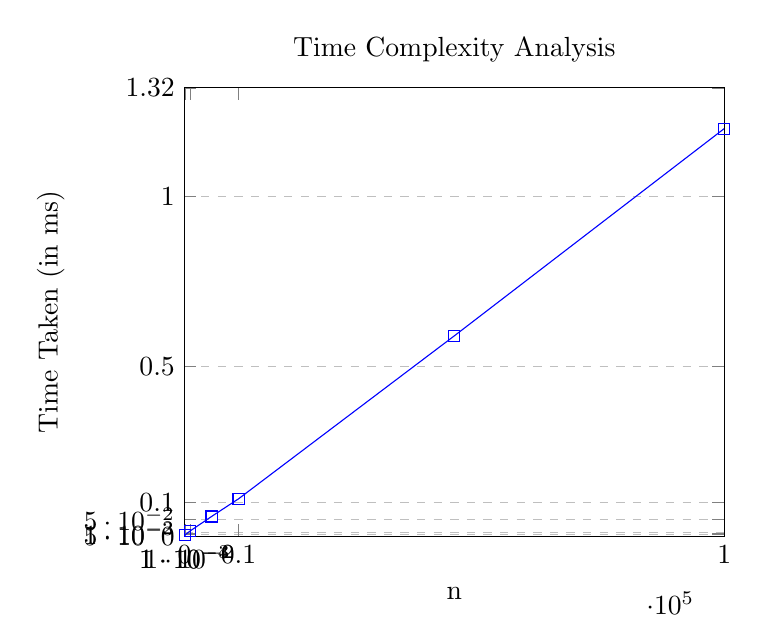
\begin{tikzpicture}
\begin{axis}[
    title={Time Complexity Analysis},
    xlabel={n},
    ylabel={Time Taken (in ms)},
    xmin=0, xmax=100000,
    ymin=0, ymax=1.32,
    xtick={0,10,100,1000,10000,100000,1000000},
    ytick={0,0.005, 0.01,0.05, 0.1,0.5,1,1.32},
    legend pos=north west,
    ymajorgrids=true,
    grid style=dashed,
]

\addplot[
    color=blue,
    mark=square,
    ]
    coordinates {
    (10,0.003)(100,0.0039)(1000,0.015)(5000,0.058)(10000,0.11)(50000,0.59)(100000,1.2)
    };
    
\end{axis}
\end{tikzpicture}

\paragraph{Alternative Algorithm:}

An alternative algorithm can be proposed which is based on the minimum cell algorithm. In this algorithm, we choose the least cost in the given row. If the supply is greater than 0, we satisfy the demand associated with that column. If the supply is zeroed, we move to the minimum in the next row, else we find the next smallest element in the same row. We continue this procedure until all the demands are satisfied. This has the same time complexity of O(n) and space complexity of O(n).

\section*{CONCLUSION}

So, with the north-west corner algorithm and its profiling, we come to the conclusion that this classical problem of minimum cost in the optimal transport problem has best time complexity of O(n) and space complexity of O(n).

\section*{REFERENCES}

\begin{enumerate}
\item Transportation Problem:\\
https://www.geeksforgeeks.org/transportation-problem-set-1-introduction/
\item Introduction to Algorithms by Cormen,Charles, Rivest and Stein.\\
https://web.ist.utl.pt/~fabio.ferreira/material/asa
\end{enumerate}\\

\newpage
\section*{APPENDIX}
\textbf{To run the code, follow the following procedure:}
\begin{enumerate}
    \item Download the code(or project zip file) from the github repository.
    \item Extract the zip file downloaded above.
    \item Open the code with any IDE like Sublime Text, VS Code, Atom or some online compilers like GDB.
    \item Run the code following the proper running commands(vary from IDE to IDE)
    \begin{enumerate}
        \item \textbf{For VS Code:} Press Function+F6 key and provide the input on the terminal.
        \item \textbf{For Sublime Text:} Click on the Run button and provide the input.\\
    \end{enumerate}
\end{enumerate}
\textbf{Code for Implementation is:}
\lstset { %
    language=C++,
    backgroundcolor=\color{black!5},
    basicstyle=\footnotesize,
}

\begin{lstlisting}
#include <bits/stdc++.h>
using namespace std;

int main()
{
	int arr[100][100];
	int n;
	cout<<"Enter n: ";
	cin>>n;
	int demand[n];
	int supply[n];
	cout<<"\nGenerated cost matrix: \n";
	for(int i=0;i<n;i++)
	{
		for(int j=0;j<n;j++)
		{
		 arr[i][j] = rand() % 9 + 1;
		 cout<<arr[i][j]<<"  ";
		}
		cout<<endl;
	}
	cout<<endl;
	for(int i=0;i<n;i++)
	{
		demand[i] = rand() % 250 + 1;
		supply[i] = demand[i];
	}
	shuffle(demand,demand+n,
	    default_random_engine(0));
	cout<<"\nDemands: ";
	for(int i=0;i<n;i++)
	{
		cout<<demand[i]<<" ";
	}
	cout<<endl;
	cout<<"\nSupply: ";
	for(int i=0;i<n;i++)
	{
		cout<<supply[i]<<" ";
	}
	cout<<endl;
	
	int i=0,j=0,cost=0;
	cout<<endl;
	while(i!=n && j!=n)
	{
		if(demand[i]==supply[j])
		{
		 cost+= demand[i]*arr[i][j];
		 i++;
		  j++;
		 demand[i] = 0;
		 supply[j] = 0;
		}
		else if(demand[i]<supply[j])	
		{	
		 supply[j]-=demand[i];
		 cost+= demand[i]*arr[i][j];
		 demand[i] = 0;
		 i++;
		}
		else if(demand[i]>supply[j])
		{
		 demand[i]-=supply[j];
		 cost+= supply[i]*arr[i][j];
		 supply[j]=0;
		 j++;
		}
	}
	cost+=demand[n-1]*arr[i-1][j-1];
	demand[n-1] -=supply[n-1];
	supply[n-1] = 0;
	cout<<"Final cost: "<<cost<<endl;
	return 0;
}
\end{lstlisting}
\end{multicols*}
\clearpage

	
\end{document}